\chapter{Fundamentals and Related Works}
\label{cha:fundamentals}
For context it is important to elaborate some basics about web components and the frameworks they are used in. This means going into the basic architecture of each framework, comparing the structure of their web components, and those created in StencilJs.//

\section{Web Components}
A basic web component is a JavaScript file that defines an encapsulated piece of HTML, CSS and JavaScript code which can be interpreted by a web browser and treated as an HTML element like <p> or <div>. Optionally, styling can also be provided via an external CSS file. This basic form of a web component does not depend on any framework and can be imported either in JavaScript, using an import command, or in HTML, using a <script> tag. In this Thesis the terms "web component" and "component" will be used synonymously.

\section{Angular}
Angular is a framework for frontend web development and was created by Google in 2010. It is described in the official documentation as a Typescript based platform that includes a framework to build web applications, as well as many helpful libraries and tools to streamline the entire process of developing and maintaining a web application [1]. This means that Angular is not just a framework, but also has a large number of tools around the framework itself.

\subsection{Components in Angular}
While basic web components in JavaScript are complicated to implement, Angular components use TypeScript and are divided into multiple files for more structure:

\begin{itemize}
\item A Typescript file for the component’s class (i.e. myComp.component.ts)
\item An HTML file for the visual representation (i.e. myComp.component.HTML)
\item an SCSS file for styling (i.e. myComp.component.scss)
\item a spec.ts (Typescript) file for testing purposes (i.e. myComp.spec.ts)
\end{itemize}
These files are linked together using the metadata given in the component.ts file.

\subsection {Basic Concepts}

\subsubsection {Services}
A service is an independent block of code that defines a specific behavior or functionality and is, in the case of Angular, written exclusively in Typescript. Services can be injected into components to provide functionality. This promotes modularity and reusability.

\subsubsection{NgModules}
A module in Angular represents a collection of components and services that share a certain context (i.e. a library of different button components).

\subsubsection{Decorators}
An angular component is implemented as a Typescript class which can contain decorators with a certain type. A decorator tells the angular compiler how to use the following code (for example, @NgComponent tells the compiler that the following class is a component).

\subsubsection{Metadata}
Metadata can be passed to a decorator to provide additional information. For example, the @NgComponent decorator’s metadata contains the location of the component’s HTML and CSS files. This way all files can be linked to a single component.

\subsubsection{Templates}
Templates are an enhancement of HTML featured in modern JavaScript/TypeScript frameworks that allows a developer to inline some functionality like hiding UI-Elements, which would normally take several additional lines of Typescript and CSS. It works by placing HTML code in a <template> tag. The UI element(s) can then be altered using event binding.

\subsubsection{Event Binding}
Event binding is a way of responding to DOM events inside the HTML code. A good example for this is the click event. By using it inside an HTML element like this:
\begin{Verbatim}[frame=single]
 <button (click)="onClick()">Do something</button>
\end{Verbatim}
Note that "(click)" is an Angular specific syntax. The button will call the onClick function in the Typescript class of the component, when it is clicked. The data flow of event binding goes only from the HTML to the TypeScript class, or from child component to parent component.
\pagebreak
\subsubsection{Property Binding}
With property binding, dynamic data can be passed to a child element of a component. This is useful for displayed data that may change frequently. For example, the path of an img tag, that has to display a different image in certain intervals can be passed with the following code:\\[0.5cm]
HTML element:
\begin{Verbatim}[frame=single]
 <img [src]="imageUrl"></img>
\end{Verbatim}
In the TypeScript file there is a variable that contains the current path.
\begin{Verbatim}[frame=single]
 imageUrl:string = '../../images/picture.png'
\end{Verbatim}

\subsubsection{Directives}
Directives are also Typescript classes that are defined with the @Directive decorator and can be attached to DOM elements in order to apply a certain behavior like changing the background color of a button while it is clicked. Directives are modular and can be used multiple times.\\\\
The graph below describes how these concepts work together. \\[0.5cm]
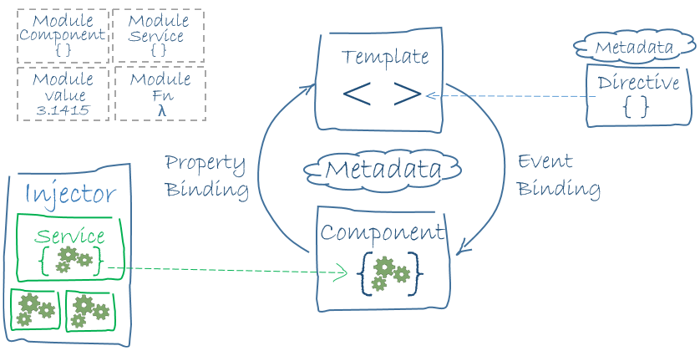
\includegraphics [height=8cm, width=15cm] {images/angular-component-structure}
\pagebreak

\subsubsection{Example of an Angular Component:}
Here is an Example of the essential files of an Angular component:\\\\
\textbf{component.html:}
\begin{Verbatim}[frame=single]
 <h1>{{text}}</h1>
\end{Verbatim}
\textbf{component.ts:}
\begin{Verbatim}[frame=single]
 @NgComponent({
   selector:'my-text',
   templateUrl: './my-text.component.html',
   styleUrls: ['./my-text.component.css']
 })
    
   export class myText{
   myText:string
 }
\end{Verbatim}
The @NgComponent decorator tells the compiler that the following class belongs to a component. The decorator takes an object as a parameter, which provides essential metadata for the component. The selector determines the name with which the component can be used in an HTML file, the templateUrl contains the path of the component.HTML file and the styleUrls is an array, in which the paths to all the CSS files belonging to the component are stored. The following class contains the variable that is used to pass text to the h1 element in the component.html file.
%xxxxxxxxxxxxxxxxxxxxxxxxxxxxxxxxxxxxxxxxxxxxxxxxxxxxxx
\section{React}
React is an open source Library for building user interfaces, released by Facebook in 2013 to make the development of their social media platform easier. React is not a fully fledged framework, because it does not dictate any design system or even provide an eco-system or built in features. Much of the functionality of a React application must be drawn from third party libraries.

\subsection{Components in React}
In Angular technologies are artificially separated by having a file for HTML and TypeScript in a component. React however separates concerns, meaning that what belongs together is stored together resulting in single file components that contain the TypeScript code as well as the CSS styling and the HTML code. To achieve this, React uses JSX or TSX, depending on whether the project is built in JavaScript or TypeScript. In this thesis TSX will be used. Furthermore, in React, components can be implemented as either class components or functional components. Before React 16.8 a class component would be required for state management. However Since update 16.8, which introduces hooks (more on hooks later) the difference between functional and class components is only syntactical and it is recommended to use functional components going forward. In contrary to Angular, React components are not updated, but created as new instances.\\[0.5cm]
In the following examples the syntactical difference between class and functional components will be demonstrated. In both cases the HTML will look like this:
\begin{Verbatim}[frame=single]
 <MyText input="Hello, World!"/>
\end{Verbatim}
\textbf{Example of a functional Component:}
\begin{Verbatim}[frame=single]
 function MyText(props:myTextProps){
   return (<h1>{myTextProps.input}</h1>);
 }
\end{Verbatim}
\textbf{Example of a Class Component:}
\begin{Verbatim}[frame=single]
 class MyText extends React.Component{
   render(){
     return(<h1>{this.props.input}</h1>)
   }			
 }
\end{Verbatim}
Note that there is no props object explicitely passed to the class. This is because the props object is auto generated by React from the HTML code.
\subsection{Basic Concepts}
\subsubsection{TSX}
Without TSX every HTML element has to be created by calling the React.createElement function or as an object. TSX is an abstraction of TypeScript that enhances the syntax and enables the TypeScript compiler to parse HTML code inside a TypeScript file into calls of the React.createElement function. Thus Typescript and HTML code can be stored in the same file. In TSX, a React component has a method called "render" which returns the HTML code to be rendered.\\\\
\textbf{Example for React.createElement call:}
\begin{Verbatim}[frame=single]
 const element = React.createElement(
   h1,
   {className: 'greeting'},
   'Hello World!'
 );
\end{Verbatim}
\pagebreak
\textbf{Example for element as object:}
\begin{Verbatim}[frame=single]
 const element = {
   type: 'h1',
   props: {
     classname: 'greeting',
     children: 'Hello, World!'
   }
 };
\end{Verbatim}
\textbf{Example of render function in TSX:}
\begin{Verbatim}[frame=single]
 render() {
   return (
     <h1>Hello, World!</h1>
   )    
 }
\end{Verbatim}
\subsubsection{States}
In React, a component maintains its own data using a state. A state is different to props in that the data is private and managed only by the component itself.
By giving the component control over its own data it can rerender itself and does no longer need to be reinstantiated every time the data changes. Since React 16.8 the use of a state no longer requires a class component with a constructor, essentially making class components obsolete. An example will be given in the hook section.\\

\pagebreak
\subsubsection{Hooks}
Hooks were introduced in React 16.8 and are JavaScript functions that are used to handle state data in components. They  extract the stateful logic from components and make it reusable. The basic Hooks are:
\begin{itemize}
\item \textbf{useState():} is used to update a state, triggering a rerendering of the component. This example demonstrates the use of useState:
\begin{Verbatim}[frame=single]
 function Counter(){
   const [count, setCount] = useState(0);
   return (
     <div>
       <p>{count}</p>		            
       <button onClick={() => setCount(count + 1)}>+</button>
     </div>
   );
 }
\end{Verbatim}
The count variable is used as the state here. The Array defines the variable and a function that can be called to change the value of count. The useState hook (more on hooks below)is used to add the state to the component and initialize it. When the button is clicked, it will use the setCount function to update the state, which will in turn cause the component to rerender with the new state.
\item \textbf{useEffect():} useEffect always runs when any stateful data changes. This behavior can be controlled more accurately by providing the hook with an array of dependencies, in which the exact states that the hook should watch for changes are specified. If useEffect is called with no dependency array, it will run when the component is mounted into the UI and when the state changes. An empty dependency array will cause the hook to only run once when the component is initialized since there are no states being watched. If the array has dependencies only those states will be watched for changes and the hook will not necessarily run upon mounting the component.\\This example shows the same component as before with a second state variable and a useEffect hook:
\begin{Verbatim}[frame=single]
 function Counter(){
   const [count, setCount] = useState<number>(0);
   const [loaded, setLoaded] = useState<boolean>(false);
   
   useEffect(
     ()=>{
       fetch('foo').then(()=>setLoaded(true))
     },
     [count] // dependency array
   )
   return (
     <div>
       <p>{count}</p>		            
       <button onClick={() => setCount(count + 1)}>+</button>
     </div>
   );
 }
\end{Verbatim}
\pagebreak
\item \textbf{useContext():} The useContext hook allows for stateful data to be shared or scoped using React's Context API. This means that a variable can be used by multiple disconnected components and, if there is a change, all the components that use the variable are updated. To do this, a variable or set of variables must be declared in the top most parent component (i.e. the App component if the data is to be used everywhere). Any child component inside the resulting component tree will inherit this variable without the need to pass it via property. By calling the useContext hook the data can be accessed and, should it change, the changes will be applied to all child components automatically. The following example demonstrates the use of useContext.\\[0.5cm]
In App.js:
\begin{Verbatim}[frame=single]
 const fruits = { //data for context
   monday: 'Apple',
   tuesday: 'strawberry'
 }
 //creating context
 const FruitContext fruits = createContext(fruits)

 function App (props) {
   return (
     //the context is shared to all components inside the
     FruitContext tag.
     <FruitContext.Provider value = {fruit.monday}>
       <todays-fruit/>
     </FruitContext.Provider>
   );  
 }
\end{Verbatim}
In todays-fruit component
\begin{Verbatim}[frame=single]
 function todays-fruit () {
   const todaysFruit = useContext(FruitContext)
   return <p>{todaysFruit}</p>
 }
\end{Verbatim}
\end{itemize}

\subsubsection{Other Concepts}
Services, decorators and metadata have already been covered in the Angular section and are not much different in React.
\section{Vue}
Vue is a very simple frontend web framework created by ex-Google employee Evan You in 2014 with the goal of building a custom tool around the best parts of Angular. Vue is designed for creating smaller projects and can be used to create entire applications or just single widgets to be used in other websites.

\subsection{Copmonents in Vue}
Vue uses single file copmonents, meaning that all the code of a component is stored in a single file. While styling can be done externally in both Angular and React, this is not the case in Vue.\\[0.5cm]
The structure of a Vue component is much simpler than in React as it is divided into three HTML tags: template, script and style. The template tag contains the HTML code of the component while the script tag contains any JavaScript or TypeScript and the style tag contains the CSS styling.\\[0.5cm]
\textbf{Example of a simple Vue component}
\begin{Verbatim}[frame=single]
 <template>
   <h1>Hello, World!</h1>
 </template>  

 <script lang="ts">
   import { defineComponent } from 'vue';

   export default defineComponent({
     name: 'hello-world',
   });
 </script>

 <style scoped>
   h1{color: green;}
 </style>

\end{Verbatim}
\subsection{Basic Concepts}
\subsubsection{Props}
Properties of a component are declared in the script tag as either an array or an object named "props". If an array is used it contains only the names of the properties as strings. these properties do not have a fixed type and cannot be configured any further. By using an object it is possible to give the property a type and configure it (i.e. make it a required property among other things). In the object the properties are stored as nested objects that contain the property's configuration.\\
\textbf{Example of Properties in a Vue component:}
\begin{Verbatim}[frame=single]
 .
 .
 .
 <script lang="ts">
   import { defineComponent } from 'vue';

   export default defineComponent({
     name: 'HelloWorld',
     props: {
       msg: {
         type: string,
         required: true
       }
     }
   });
 </script>
 .
 .
 .
\end{Verbatim}
\subsubsection{Property binding}
The Vue equivalent of Angular's property binding is the v-bind directive. On a surface level, the difference is only syntactical. By putting \verb+"v-bind:"+
before a property of an HTML element, variables can be assigned to the property.\\
\textbf{Example of the v-bind directive:}
\begin{Verbatim}[frame=single]
 <hello-world v-bind:msg="{{message}}"\>
\end{Verbatim}
\subsubsection{Registration}
When the Vue compiler comes across a component inside a template tag it needs to know where to find the corresponding component file in order to render the component. Therefore a component must always be registered in its parent component. This is done via an object in a component's script tag that contains the names of all the components used in the component's template.
Components can be registered either globally by using the app.component function or locally using the approach described above.

\section{Stencil}
Stencil is an open source library created by the ionic framework team specificly to create web components that could be used in Angular, React and Vue using a single code base as ionic supports all three of these frameworks and provides a library of components out of the box that need to run in each framework. As mentioned, the purpose of Stencil is only to create component libraries and not full websites or apps. There is an Index.html file in a Stencil project, but it is only meant for testing. Therefore Stencil is not considered a framework. The most important part of Stencil are two features. The first is it's compiler which creates framework agnostic web  components, meaning pure JavaScript components along with SCSS files for styling. The second is the "output targets" feature which can produce framework native components.

\subsection{Components in Stencil}
Components in Stencil are written in TSX (more on TSX in the React chapter) with a separate CSS file. The structure of the component itself is very simple. The component is just a TypeScript class with a component decorator which holds metadata. Inside the Class most of a component's functionality that is not a private function uses a decorator.

\subsection{Basic Concepts}
\subsubsection{Most Common Decorators}
In Stencil most functionalities are declared via a decorator. The most common ones are:
\begin{itemize}
\item \textbf{@Component:} The following class is a component.
\textbf{Example:}
\begin{Verbatim}[frame=single]
   @Component({
     tag: 'hello-world',
     styleUrl: 'hello-world.CSS'	
   })
\end{Verbatim}
\item \textbf{@Method:} The following function is a public Method.\\
\textbf{Example:}
\begin{Verbatim}[frame=single]
 @Method()
 toString():string {
   return 'Hello, World!';
 }
\end{Verbatim}
\item \textbf{@Prop:} Declares a property of the component that can be used for passing data to the component via HTML.
\item \textbf{@Event:} Creates an event emitter that takes data as a parameter and can emit DOM events.\\
\textbf{Example:}
\begin{Verbatim}[frame=single]
	@Event buttonClicked: EventEmitter<string>
	
	onButtonClick(string s) {
		buttonClicked.emit(s);
	}
\end{Verbatim}
\item \textbf{@Listen} Creates an EventListener that is triggered by a specified event and executes a given function.
\textbf{Example:}
\begin{Verbatim}[frame=single]
 @Listen('HelloButtonClicked') 	
 helloButtonClickHandler(event: CustomEvent<string>) {
   console.log('Hello, World!')
 }
\end{Verbatim}
\item \textbf{@Watch:} Stencil's equivalent of useEffect. The Watch decorator reacts to changes of states or props and executes a function that is implemented immediately after it. The Watch decorator also takes the old value as well as the new value of the watched data as a parameter.
\textbf{Example:}
\begin{Verbatim}[frame=single]
 @State() displayText: string;
 
 @Watch('displayText')
 watchStateHandler(oldValue:string, newValue:string){
   console.log('the old value was: ', oldValue);
   console.log('the new value is: ', newValue);
 }

 onButtonClick(string s) {
   buttonClicked.emit(s);
 }
\end{Verbatim}
\end{itemize}



